%% 
%% Copyright 2019 Elsevier Ltd
%% 
%% This file is part of the 'CAS Bundle'.
%% --------------------------------------
%% 
%% It may be distributed under the conditions of the LaTeX Project Public
%% License, either version 1.2 of this license or (at your option) any
%% later version.  The latest version of this license is in
%%    http://www.latex-project.org/lppl.txt
%% and version 1.2 or later is part of all distributions of LaTeX
%% version 1999/12/01 or later.
%% 
%% The list of all files belonging to the 'CAS Bundle' is
%% given in the file `manifest.txt'.
%% 
%% Template article for cas-dc documentclass for 
%% double column output.

%\documentclass[a4paper,fleqn,longmktitle]{cas-dc}
\documentclass[a4paper,fleqn]{cas-dc}

%\usepackage[authoryear,longnamesfirst]{natbib}
\usepackage[authoryear]{natbib}
%\usepackage[numbers]{natbib}

%%%Author definitions
\def\tsc#1{\csdef{#1}{\textsc{\lowercase{#1}}\xspace}}
\tsc{WGM}
\tsc{QE}
\tsc{EP}
\tsc{PMS}
\tsc{BEC}
\tsc{DE}
%%%

\begin{document}
\let\WriteBookmarks\relax
\def\floatpagepagefraction{1}
\def\textpagefraction{.001}

\shortauthors{Halil \.{I}brahim \c{C}elenli et~al.}
%\shortauthors{Author 1} 

\title [mode = title]{A new document vector representation using word2vec and latent dirichlet allocation} 

\author[1]{Halil \.{I}brahim \c{C}elenli}[orcid=0000-0001-5369-9677]     
%\author[1]{Author 1} [orcid=0000-0000-0000-0000]   
\cormark[1]
\ead{email@gmail.com}
\ead{halilibrahimcelenli@gmail.com}
%\cortext[cor1]{Corresponding author}
%\author[1]{Author 2}
%\author[2]{Author 3}

\author[1]{Sevin\c{c} \.{I}lhan Omurca}
\author[2]{Murat Can Ganiz}

%\address[1]{Address 1}
%\address[2]{Address 2}


\address[1]{Department of Computer Engineering, Faculty of Engineering, Kocaeli University, Kocaeli, Turkey}
\address[2]{Department of Computer Engineering, Faculty of Engineering, Marmara University, İstanbul, Turkey}



\begin{abstract}
	Word embedding models typically learn a vector representation for each word, based on the co-occurrence statistics in the contexts across a text corpus. On the other hand, topic modeling techniques produce a distribution over words for each latent topic and a distribution over latent topics for each document in a given corpus. We combine word embedding models with topic models for a better semantic representation which in turn used to represent documents. To demonstrate the value of our approach we choose document categorization as the mainstream NLP task. We compare the classification performance of well-known  machine learning classifiers on the proposed document vectors and traditional Doc2vec approach. We show that the proposed document vectors; combination of Word2vec and LDA improves the classification results and reduce the complexity of the resulting model.
	
\end{abstract}

\begin{graphicalabstract}
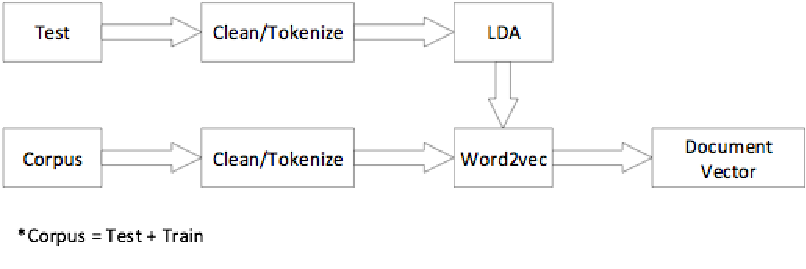
\includegraphics{figs/fig7.pdf}
\end{graphicalabstract}

\begin{highlights}
    \item We present TopWord2vec, a combination of Word2vec and LDA models
	\item TopWord2vec model gives better results than the Doc2vec model.
	\item TopWord2vec model gives good results in tweets and news datasets.
	\item TopWord2vec model improves the classification results and reduces the complexity of the results.
\end{highlights}

\begin{keywords}
	Natural language processing \sep Text Classification \sep Word embeddings \sep Topic modeling \sep LDA \sep Doc2vec
\end{keywords}


\maketitle



\section{Introduction}


Since the natural language; text documents are unstructured they need to be converted into structured format such as vectors or matrices. This preprocessing stage; the representation of words or documents is crucial because this process may have a fundamental effect on the performance of the Natural Language Processing (NLP) tasks such as document classification.  In this study we focus on creating a novel document representations by combining word embedding models with topic models. We evaluate the value of this approach in document classification domain. The aim of document classification is to assign the most appropriate label to a document from a set of predetermined labels. Many document classification approaches use bag-of-words (BoW) representations which results in usually very high dimensional and sparse vectors. Especially the sparsity creates several problems for machine learning algorithms that operate on these representations. They ignore the semantic relationships between different words and therefore the documents \citep{ref1}. The generalization power of the classification models become stronger when they make use of the semantic information.  

Recently, word embedding techniques widely used to represent words as low dimensional dense vectors. These methods are capable of implicitly incorporating both semantic and syntactic similarity information into these vector representations because they employ context or co-occurrence information in a very large training corpus.  Word2vec developed by  \cite{ref2} is one of the  popular methods to learn word embeddings. Vectoral representations of words that are semantically similar lies in close proximity in the multidimensional Euclidean space as measured using a distance metric.  Similarly, doc2vec algorithm creates dense vectoral representations of documents. \cite{ref3} proposed Doc2vec algorithm to represents a document by using the word representations of the document and these representations yields higher classification accuracy than many other document representation methods for document classification tasks \citep{ref4}.

One of the unsupervised techniques to capture the semantic similarity between documents is topic modelling. Topic modelling learn latent document representations that can be used to perform text mining tasks such as classification, summarization or information retrieval. Latent Dirichlet Allocation (LDA)  \citep{ref5} which is a well-known algorithm for topic modelling, groups similar words together in topics and represents documents as distributions over these topics. The idea behind LDA is to model documents as a distribution of topics where each topic defines a distribution over words. In LDA, the distributions are assumed as Dirichlet distribution which is a continuous generalization of the multinomial distribution.

Performance of document classification systems mainly relies on quality of the document vectors. Therefore, it becomes crucial to create low-dimensional representations of documents that can capture semantic and contextual information about the corpus \citep{ref6}.

We present a new approach to document representation by merging two different document representation methods named TopWord2Vec. The first one is the doc2vec representation \citep{ref3} and the second one is the document representation based on the LDA. Our main motivation is to combine the capability of representing each document by word vectors which will incorporate co-occurrence based semantic information between words and the semantic information words, documents and latent topics that characterize the overall corpus. In our method, the latent topics of the corpus are used to enrich the semantics of the document representation. We obtain word distributions per topic and topic distribution per document using the LDA. In addition to this, all word vectors in each document in the corpus are generated by word2vec algorithm. To create a document representation we multiply LDA based vectors with the word vectors. We experimentally evaluate our approach using the doc2vec representations as the baseline document representation and based on these representations we use well-known classification algorithms such as Support Vector Machines (SVM), k-Nearest Neighbor (KNN), Random Forest (RF), Bernoulli Naive Bayes (BNB) and Logistic Regression (LDA). Experiments show that, by using our proposed document representation approach classification algorithms can achieve higher prediction accuracy values. Furthermore, considering the training times, our approach is faster than doc2vec.

We also investigate the impact of choosing different numbers of topics on the proposed approach. The perplexity which is the measure of the ability of a model to generalize to unseen data \citep{ref7} is used to adjust the topic numbers to input the LDA.
The remaining part of this paper is organized as follows: Section 2 gives related work on the use of word embeddings and topic modeling methods. LDA, word2vec and doc2vec are briefly introduced in section 3. In section 4, our proposed model is described. Experimental setup and results are given in section 5 and section 6. section 7 concludes the paper with a discussion and conclusions.

\section{Related Work}

Distributed vector representation of words or paragraphs in a continuous space is highly popular in text mining systems lately \citep{ref8}. One of the inspirational approaches is \citep{ref9} neural language model which is constituted as a feed forward neural network with a linear projection layer and a non-linear hidden layer. This model learns distributed representations for words. Recurrent Neural Network (RNN) based language model  \citep{ref10} emphasize the major deficiency of a feed-forward network that has to use limited size of context that needs to be specified before training. To address this, the Recurrent Neural Network Language Model (RNNLM) is presented by \cite{ref10}. This propose a neural network architecture to establish semantically better represented word embeddings by using local and global contexts in learning. Doc2vec approach is proposed by \cite{ref3} in which they present an unsupervised algorithm that learns fixed-length vector representations from variable length of texts such as paragraphs. They show that the paragraph vector is adequate in capturing the semantics of paragraphs and has ability to overcome many weaknesses of bag-of-words models. Doc2vec model trains a paragraph vector by a linear combination of the word embeddings. \citep{ref11} proposed GloVe model which captures global corpus statistics directly. To achieve this, they trained a specific weighted least squares model on global word-word co-occurrences.

Although the above mentioned methods have all good performances compare to the traditional bag-of-words models there is still room for improvement. One of the interesting approaches for this is to integrate LDA and word embeddings for a better word or document representation. 

\cite{ref3} propose an unsupervised framework that learns continuous distributed vector representations for different sizes of paragraphs. The paragraph vector can be considered as a memory that remembers what the topic of the paragraph is. This unsupervised method is called as Distributed Memory Model of Paragraph Vectors (PV-DM) due to emphasize that their method can be applied to any phrase, sentence or paragraph. In this method, paragraph vectors are unique among paragraphs. Although each word may have various meaning, each word corresponds to a single word embedding. This can be considered as limitation of the model due to leading to inaccurate semantic representation of paragraph \citep{ref12}. 

\cite{ref6} propose the topical word embedding model which considers each word have different embeddings under different topics. They integrate word-topic relation into word embedding model and so the model discovers the various meanings of a word across different topics. LDA and Skip-Gram \cite{ref2} models are implemented to obtain word-topic pairs and to learn topical word embeddings respectively. Their study only considers the topic diversity of words.

\cite{ref13} incorporated topics into a LSTM model, and call the resulting model Contextual LSTM. They concluded that, using topic modelling with vectors, in- stead of supervised topic models, are promising. 

\cite{ref14} extracted a topic-conditioned Recurrent neural network language models (RNNLM) by performing LDA to fixed-length block of texts. They provide the topic information directly at the input of the model.

\cite{ref1} applies word2vec to learn word vector. Then they assumed that word vectors with the same topic follow a Gaussian mixture model (GMM) that describe the distributions of all words, in which each Gaussian represents a latent topic. After text generation process, a modified GMM is used to represent texts based on their topics. The weight coefficient of GMM is calculated by the probability that the word belongs to each topic. 

\cite{ref15} show that latent feature representations can be used to improve topic models. The word-topic mapping is improved by incorporating two different Dirichlet multinomial topic models with latent feature vector representations of words trained on very large corpora.

\cite{ref16} proposed a hybrid method that combines Word2Vec and LDA to generate not only document-topic relations but also the contextual relationships among words. The performance of their model is investigated by using Support Vector Machines (SVM) on the 20NewsGroups dataset.

\section{Preliminaries}

This section introduces the relevant models such as LDA and word embeddings that are the components of the proposed system. 

\subsection{Latent Dirichlet Allocation (LDA)}

Latent Dirichlet Allocation (LDA)  \citep{ref17,ref5}  represents a document collection by their thematic content. LDA models a large collection of unlabeled documents as a mixture of topics, where each topic as a distribution over the terms of a fixed vocabulary. The graphical representation of LDA model is depicted in Figure \ref{fig1}.

\begin{figure}
	\centering
	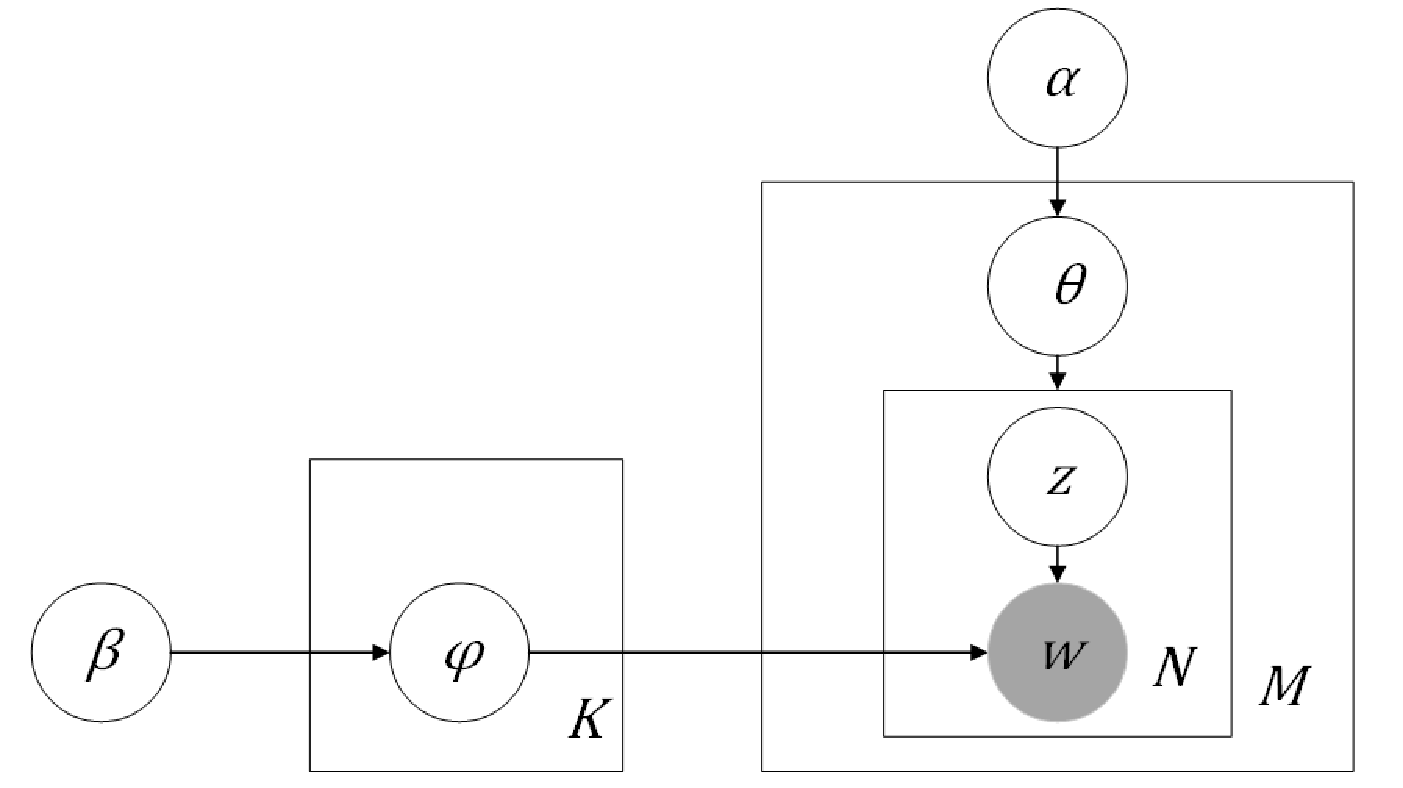
\includegraphics[scale=.3]{figs/fig1.pdf}
	\caption{A graphic representation of LDA algorithm.}
	\label{fig1}
\end{figure}

The only observable variable is represented as w, other represented variables are latent variables. z is denoted as a topic in LDA. The document-topic distribution is denoted as $\theta$ , and each one is drawn independently from a symmetric Dirichlet prior $\alpha$. The topic-word distribution is denoted as $\phi$, and each one is drawn from a symmetric Dirichlet prior $\beta$. LDA assumes that a document consists K topics, and the generative probability distribution for the documents is
\begin{equation}
	\label{eq1}
	\begin{gathered}
		p(\phi,\theta,z,w) = \phantom{sbdabdsjhbadsada} \\
		\prod_{k=1}^{K}p(\phi_k |\beta) \prod_{m=1}^{M}p(\theta_m |\alpha) \prod_{n=1}^{N}p(z_m,_n|\theta_m) (w_m,_n |z_m,_n,\phi_k ) 
	\end{gathered}
\end{equation}
To obtain the model parameters the posterior distribution is used. 
\begin{equation}
\label{eq2}
p(\phi,\theta,z|w,\alpha,\beta)=  \frac{p(\phi,\theta,z,w|\alpha,\beta)}{p(w|\alpha,\beta)} 
\end{equation}
Unfortunately this distribution is intractable to compute due to the marginal probability of the observed data in the denominator cannot be computed exactly. The Collapsed Gibbs sampling is used as an approximate inference technique in our experiments. 

\subsection{Word2vec}

Word2vec \citep{ref2} is a shallow neural network which learns low dimensional vectors from trained large text corpus. It predicts words based on their context by using Continuous Bag of Words (CBOW) or Skip-Gram models which are two distinct neural network models. CBOW model predicts the current word based on the context, on the other hand, the skip-gram predicts surrounding words given the current word \citep{ref2}. The architectures of these models are shown in Figure \ref{fig2}.  %[a] and Figure \ref{fig2} [b]. 

\begin{figure}
	\centering
	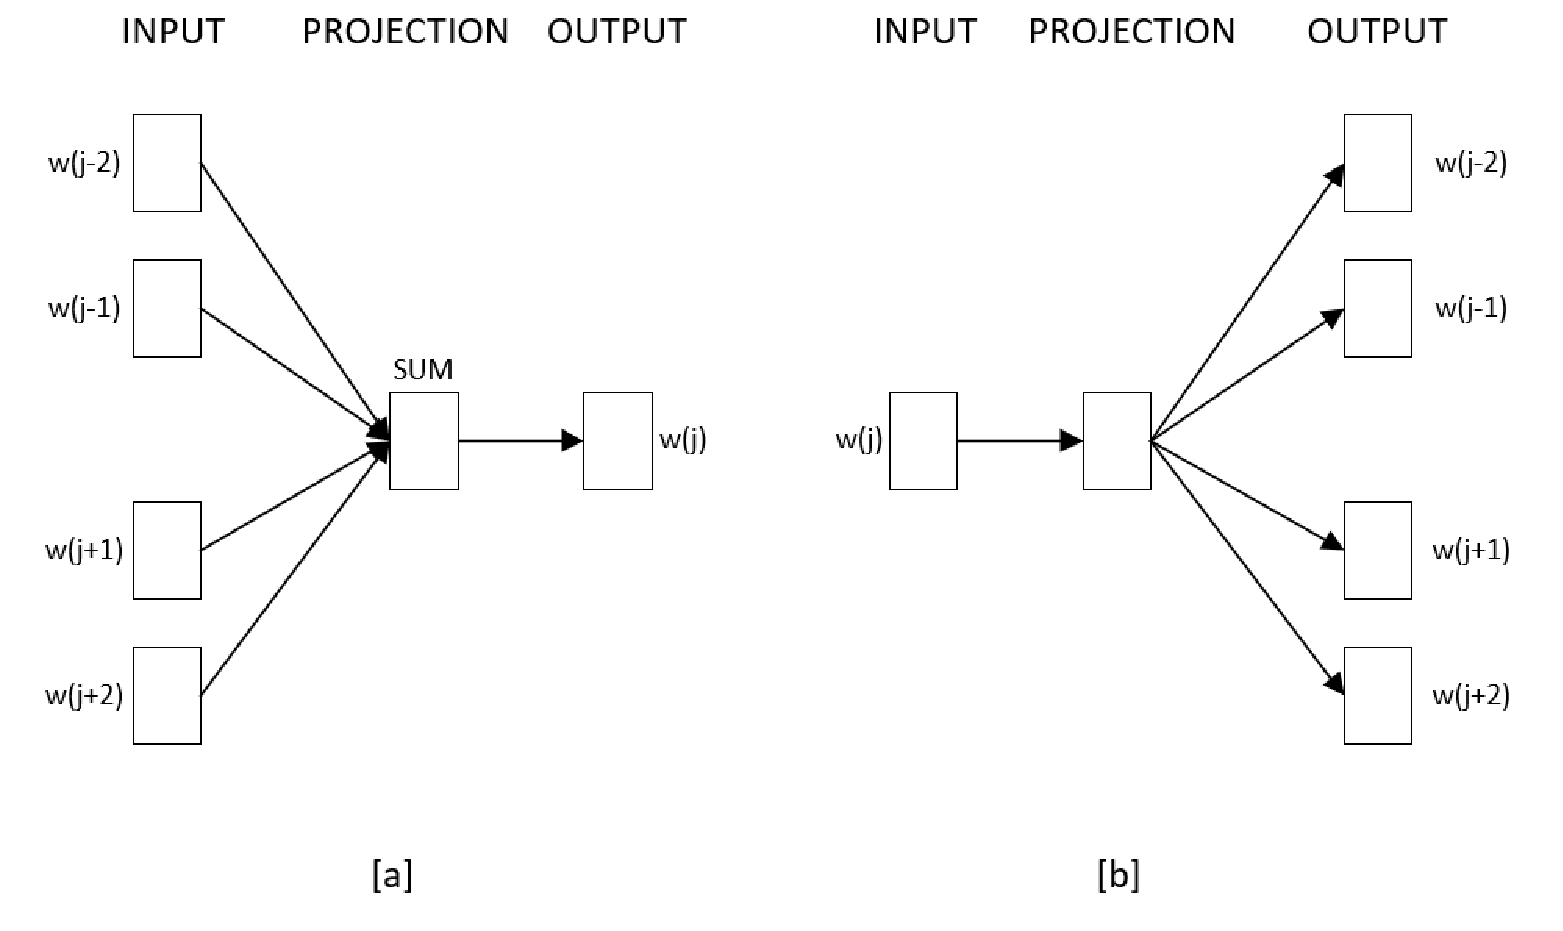
\includegraphics[scale=.3]{figs/fig2.pdf}
	\caption{ [a] CBOW and [b] Skip-gram Architectures \cite{ref2}}
	\label{fig2}
\end{figure}
Both neural models learn the underlying relationship between words and their context. By capturing the relationships between words and their context, Word2vec represent words as vectors carrying semantic information. 

In this paper, CBOW is used to learn Word vectors. CBOW model predicts a target word $w_j$ using the context words includes previous c words and behind c words of word $w_j$ in a sliding window i.e. $ C ( w_j  )= \{  w_j  - c, w_j  - c + 1, \cdots , w_j - 1, w_j  + 1, w_j + 2, \cdots , w_j  + c \}$. Given a sequence of training text $ D= \{w_1, w_2, \cdots, w_K \}$ The objective, is to maximize the average log likelihood of D. 
\begin{equation}
\label{eq3}
L(D)=\frac{1}{K} \sum_{j=c}^{K-c}\log {p(w_j | w_{j-c},...,w_{j+c})}        
\end{equation}
For the estimation part the softmax function is used. The softmax is an activation function that produces a probability-based loss value using values from artificial neural networks based deep learning algorithms. The calculation is as follows.
\begin{equation}
\label{eq4}
log {p(w_j | w_{j-c},...,w_{t+c})} =\frac{e^yw{j}}{\sum_{i}e^yi}        
\end{equation}
Calculations using y(i), which are normalized log likelihood for each output word i, are shown as Equation \ref{eq5}.
\begin{equation}
\label{eq5}
y = b+Uh(w_{j-c},...,w_{j+c};W)         
\end{equation}
In the calculation above, U and b parameters belong to softmax function. The parameter h is formed by the concatenate or averaging of the word vectors.

The purpose of using CBOW instead of skip-gram is that skip-gram calculations are slow and it requires larger amount of the training data to extract context vectors over predicted words. In addition, CBOW architecture has a better performance on the frequently used words  \citep{ref2} which in our case leads to the topics.

\subsection{Doc2vec}

Doc2vec, is a model that extracts relations between paragraph vectors. By using again a shollow neural network, the model  automatically extracts features that represent the document in a relatively low dimensional Euclidean space. In 2014, Tomas  This distributed representation of documents using dense low dimensional vectors outperform existing bag-of-words representation of documents with high dimensional, highly sparse vectors in several text mining problems \citep{ref3}.
This model has 2 different architecture which was shown under  Figure \ref{fig3} and Figure \ref{fig4} named as Distributed Memory (DM) and Distributed Bag of Words (DBOW) architecture. 
\begin{figure}
	\centering
	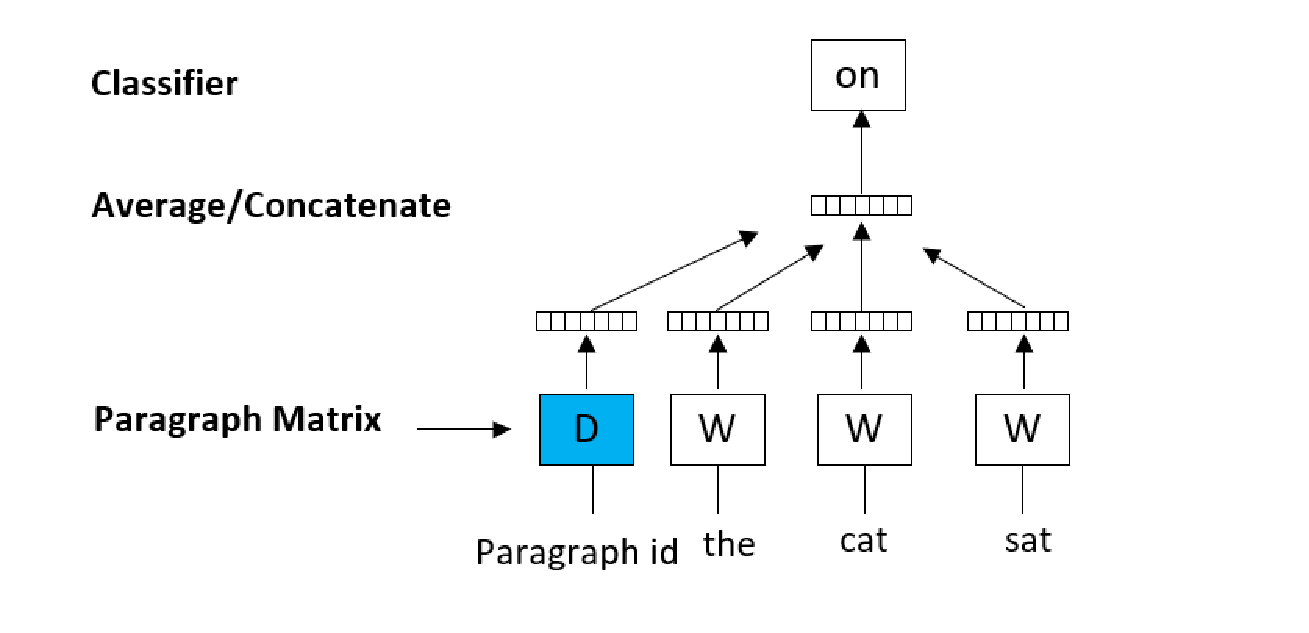
\includegraphics[scale=.3]{figs/fig3.pdf}
	\caption{Estimation of the Word “on” with Distributed Memory Architecture \cite{ref3}}
	\label{fig3}
\end{figure}
\begin{figure}
	\centering
	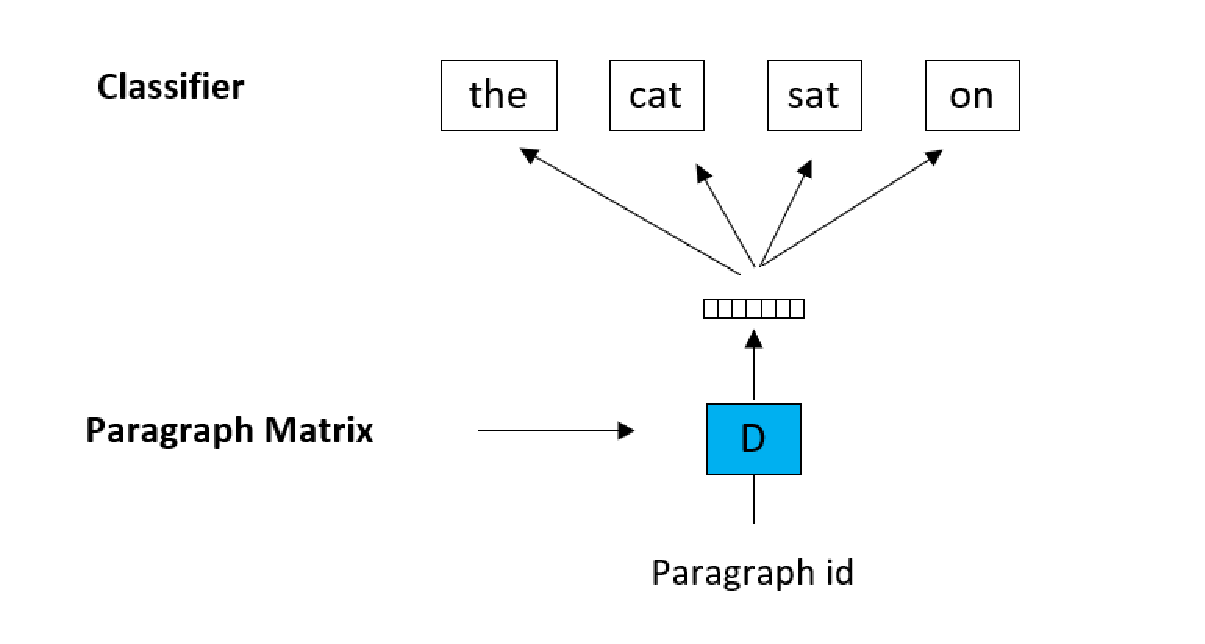
\includegraphics[scale=.3]{figs/fig4.pdf}
	\caption{Estimation of the Word "the","cat","sat","on" with Distributed Bag of Words  Architecture \cite{ref3}}
	\label{fig4}
\end{figure}
\phantom{In this paper, Distributed Memory (DM) is used to learn paragraph vectors. DM architecture was shown on Figure 3. Each paragraph is labeled with a specific paragraph id in th}
\phantom{In this paper, Distributed Memory (DM) is used to learn paragraph vectors. DM architecture was shown on Figure 3. Each paragraph is labeled with a specific paragraph id in th}
In this paper, Distributed Memory (DM) is used to learn paragraph vectors. DM architecture was shown on Figure \ref{fig3} Each paragraph is labeled with a specific paragraph id in the DM architecture. This represents the missing word and increase the success rate of the output. In this approach the correlations are being built between words instead of paragraphs. Here, the D matrix is the representation of the documents, while the W matrix is the unique column matrices used to represent the words.  
As shown below, the only difference from the y formulation through the CBOW architecture is the addition of the D matrix. Matrix D is a prediction provides based on how often and in what order the words are displayed.
\begin{equation}
\begin{split}
\label{eq6}
y = b+Uh(w_{j-c},...,w_{j+c};W,D)   
\end{split}      
\end{equation}
We can consider the architecture of the DM as the implementation of the CBOW architecture on documents. The DBOW architecture is likewise known for its similarity to skip-gram architecture. We have chosen the DM architecture as the doc2vec model because we built the proposed method on CBOW architecture.

The most important property of the paragraph and word vectors is that they are unsupervised meaning that they don't require class labels of the documents. With this method, no class labeled data is required during the training of the model.  

\section{Approach}


As a novel approach, we incorporate the results of topic modelling with the word embedding model to obtain a document vector which underlies theme of the document.  
The main steps of our proposed model are as follows:

\textbf{Step1.} The document vectors which include document-topic distributions and topic vectors which include topic-word distributions are obtained by using LDA as depicted in Figure \ref{fig5}.

\begin{figure*}
	\centering
	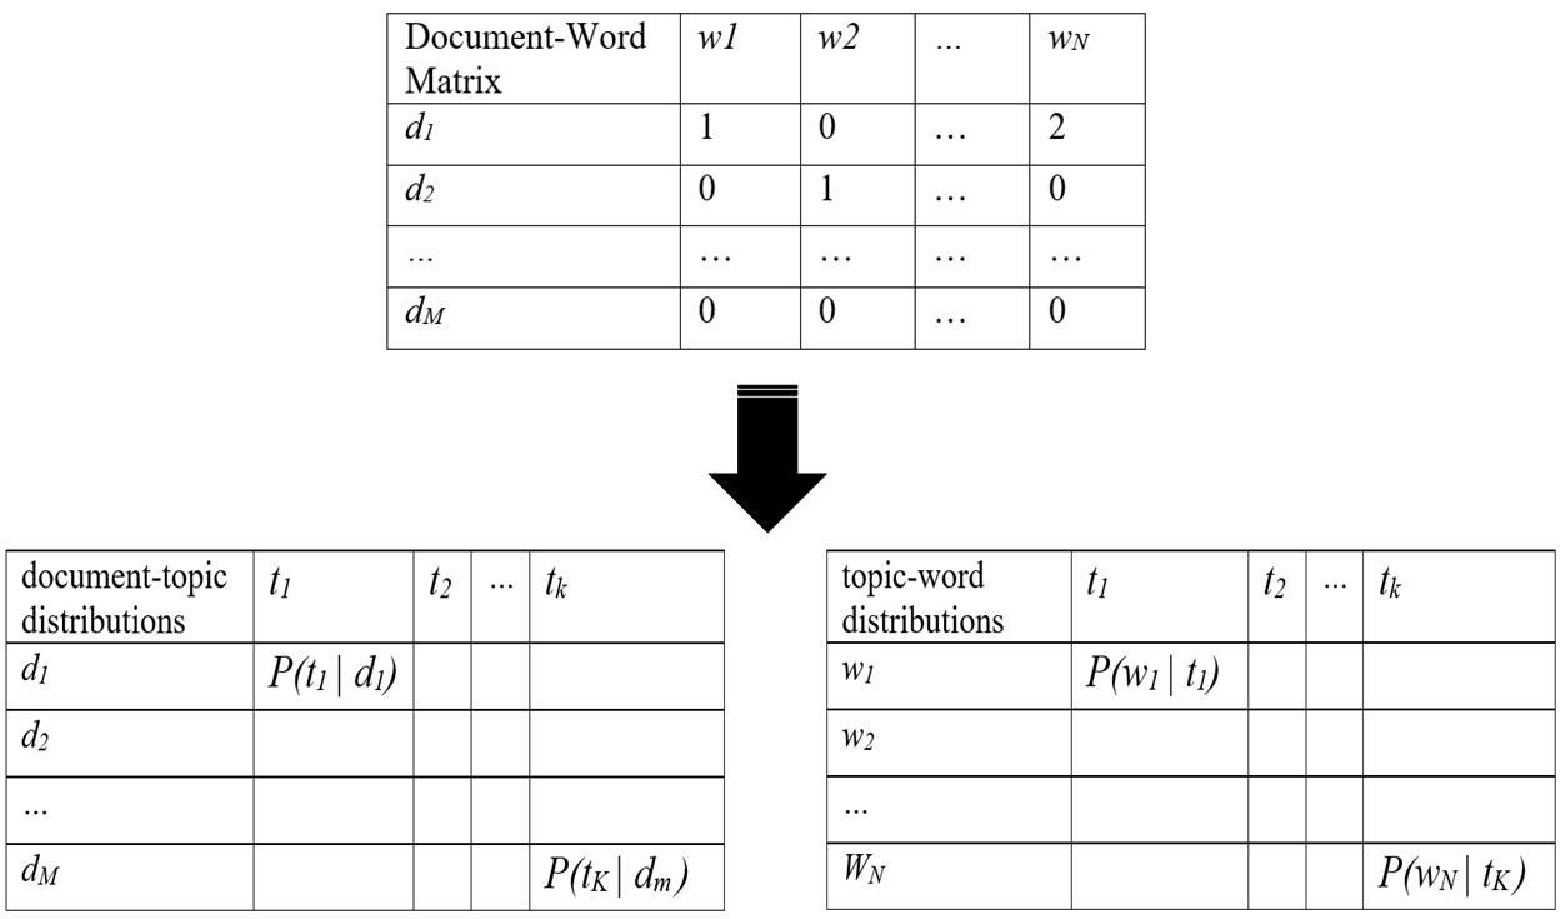
\includegraphics[scale=.4]{figs/fig5.pdf}
	\caption{Outputs of LDA: Document Vectors (document-topic distributions) and Topic Vectors (topic-word distributions)}
	\label{fig5}
\end{figure*}

Topic models are based on the simple idea that given a set of documents $D=\left\{d_1,d_2,…,d_M\right\}$ are mixtures of topics $T=\left\{t_1,t_2,…,t_K\right\}$, where a topic is a probability distribution over words $W=\left\{w_1,w_2,…,w_N\right\}$. Therefore in topic models such as LDA, how well a word represents a topic of a document can be defined with two distributions: topics’ distributions under documents which can be denoted as $(T|D)$ and the words' distributions under topics which can be denoted as $P(W|T)$. The probability term $P(T|D)$ measures the likelihood of a topic in a document, and the probability term $P(W|T)$ measures the likelihood of a word in a topic. If a document comes from a specific topic then the likelihood of a topic in that document must be maximum. If a word comes from a specific topic then the likelihood of the word in that topic must be maximum. 


For an instance, if the likelihood of a word “student” in a specific topic such as “education” is maximum then the “student” is important for reflecting “education” topic.  Besides, if the likelihood of “education” topic in a document which includes “student” is maximum then “student” is important for reflecting “education” topic for that document. 

It is assumed that, if a probability distribution of word n under topic k is maximum then the topic of that word is defined as $t_k^*$  Based on this topic information, a new weight degree which denoted as $a_n^m$ and defined as in Equation \ref{eq7} is proposed to represent the importance of word n in document m. 
\begin{equation}
\label{eq7}
t_{k^*}=\arg\max P(w_n \mid t_k ); k=1,…,K
\end{equation}
\[a_n^m= P(w_n \mid t_{k^*})\times P(t_{k^*}\mid d_m); n=1,...,N\]
The higher the value of $\alpha_n^m$, the more decisive the $w_n$ for the document m is. 

\textbf{Step2.} The word embedding vectors are obtained by using word2vec. The learned word vectors underlie relationship between words and their context. This information considered as a semantic knowledge about the words in the corpus. Word2vec vectorizes each word in corpus into a fixed length vector. 
After word2vec training, words in vocabulary is represented as
$V=\left\{v_1, v_2, ..., v_N\right\}$. 

\textbf{Step3.} The semantic representation of the words is strengthened by combining the results of the previous two steps. The numerical values of the word embedding vector obtained in the second step and the probability distributions obtained in the first step are multiplied to modify the word embedding vector. Lets $ V'=\left\{v_1' ,v_2', ..., v_N' \right\} $ represents the modified word embedding vector for document m. Modified weight of word n in document m, is obtained as in Equation \ref{eq8}. 
\begin{equation}
\label{eq8}
v_{n^I} = v_n\times\alpha_{n^m}; n=1,…,N
\end{equation}
\textbf{Step4.} At last, the document vector is created by combining  modified word vectors. Document vectors generated by summing word vectors and divide them to the numbers of words in documents afterwards as in Equation \ref{eq9}.
\begin{equation}
\label{eq9}
d_m{^I}=\frac{\sum_{v_n^I}\in d_m^{v_n^I}}{\mid d_m\mid};m=1,…,M
\end{equation}
These steps are applied to all documents in the corpus and the document vectors are obtained by our proposed approach. After the completion of these steps, document vectors and their associated class labels are used to train traditional machine learning classifiers such as SVM, KNN, Random Forest, Bernoulli Bayes and Logistic regression classifiers respectively. The proposed model is illustrated in Figure \ref{fig6}.
\begin{figure*}
	\centering
	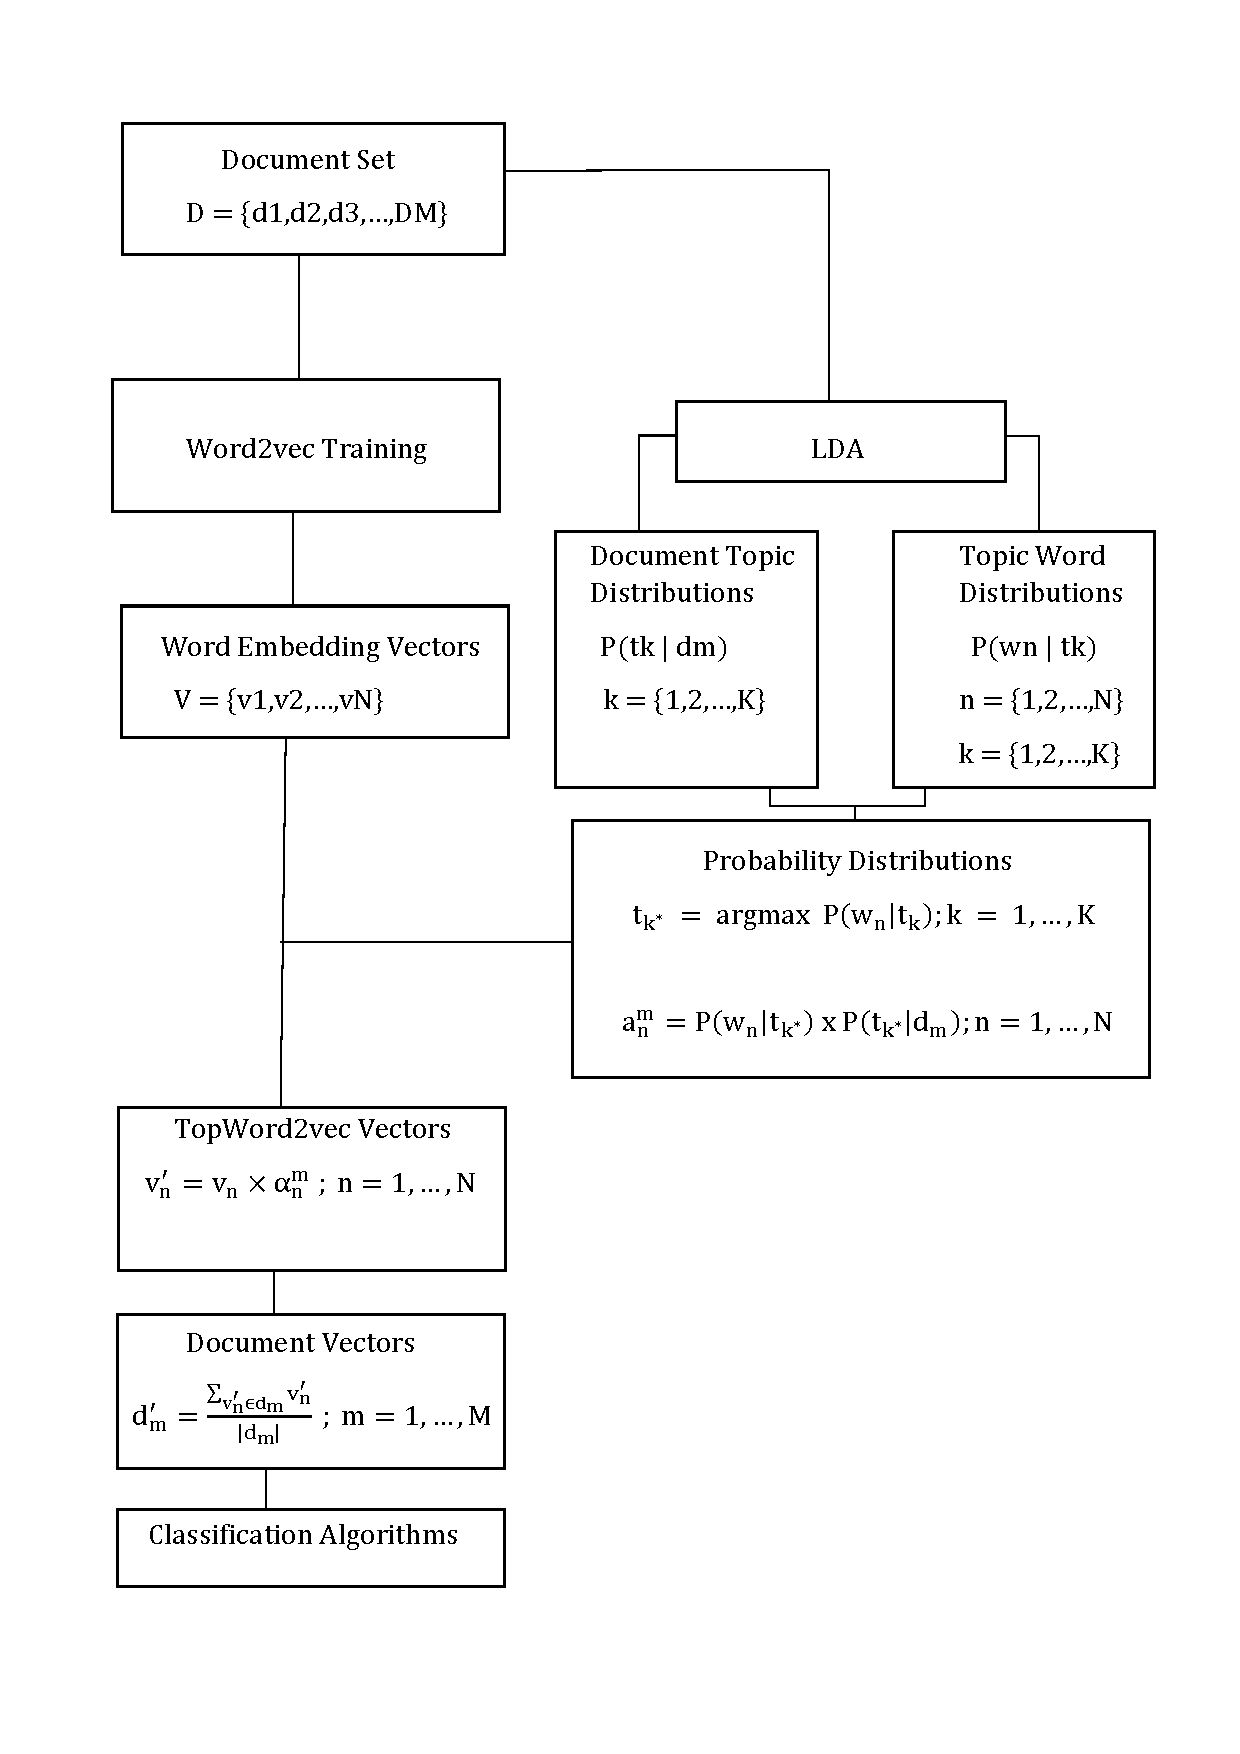
\includegraphics[scale=.8]{figs/fig6.pdf}
	\caption{The Proposed TopWord2vec Model }
	\label{fig6}
\end{figure*}

\section{Experimental Design}


\subsection{Data Sets and Preprocessing}

We use several Turkish and English text classification datasets to evaluate our approach. The Turkish Datasets used in this study are; 1150News, and 3000Tweet which are provided by Yildiz Technical University Kemik NLP Research Group\footnote{www.kemik.yildiz.edu.tr/?id=28}. We also used TTC-3600 \citep{ref18} and 9127Tweet\footnote{www.kemik.yildiz.edu.tr/?id=28}  datasets. The datasets consist of tweets such as 3000Tweet and 9127Tweet includes 12 unique words per document on average, while news documents includes 228 words per document , thus they can be considered as short text and long text datasets, respectively. 

10 million tweets are used together with four of Turkish datasets with an overall number of 10.073.869. Table \ref{tab1} summarizes the Turkish datasets used in experiments. 


\begin{table*}
	\caption{Properties of the Turkish datasets}	\label{tab1}
	\begin{tabular*}{\tblwidth}{ p{36pt}p{67pt}p{40pt}p{77pt}p{77pt} }
		\toprule
		\textbf{Dataset} & \textbf{Description} & \textbf{Number of Classes} & \textbf{\phantom{a} Vocabulary Size \phantom{a}  (Number of Words)} & \textbf{\phantom{aa}  Mean Length \phantom{aa} (Number of Words) } \\ 
		\midrule
		1150News         &  Consists of 1150 news data                             & 5             & 50.973                                                                                & 218                                                                                          \\ 
		3000Tweet          &Consists of 3.000 tweets data                              & 3               & 12.040                                                                                & 10                                                                                          \\ 
		9127Tweet           &Consists of 9.127 tweets data                              & 2               & 26.682                                                                                & 16                                                                                          \\ 
		Ttc-3600            &Consists of 3.600 news data                              & 6             & 104.774                                                                                & 239                                                                                          \\ 
		\bottomrule
	\end{tabular*}
\end{table*}


Comparing to the Turkish datasets, English datasets are only consists of tweet data. Archeage, Iphone6, Hobbit as Sent Collection Datasets and Stsgold \cite{ref19} datasets\footnote{http://lasid.sor.ufscar.br/ml-tools/} are used. There are also unlabeled tweets for training purposes. All the English datasets consists of 1.882.876 data. Table \ref{tab2} summarizes these datasets. 


\begin{table*}
		\caption{Properties of the English datasetss}	\label{tab2}
	\begin{tabular*}{\tblwidth}{ p{33pt}p{28pt}p{28pt}p{40pt}p{77pt}p{77pt} }
		\toprule
		\textbf{Dataset} & \textbf{Positive} & \textbf{Negative} & \textbf{Sum Data} & \textbf{\phantom{a} Vocabulary Size \phantom{a}  (Number of Words)} & \textbf{\phantom{aa}  Mean Length \phantom{aa} (Number of Words) } \\ 
		\midrule
		Archeage         & 724               & 994               & 1.718             & 2.945                                                                                & 13                                                                                          \\ 
		Iphone6          & 371               & 161               & 532               & 1.439                                                                                & 10                                                                                          \\ 
		Hobbit           & 354               & 168               & 532               & 1.311                                                                                & 13                                                                                          \\ 
		Sts-gold         & 632               & 1.402             & 2.034             & 4.609                                                                                & 12                                                                                          \\ 
		\bottomrule
	\end{tabular*}
\end{table*}



The process starts with the preprocessing steps. During preprocessing, punctuation, numerical characters and stopwords are removed. Stemmer is not used. After the completion of data preprocessing, the tokenized words in test data and corpus data are sent to LDA and Word2vec respectively.  Finally, by combining LDA with Word2vec model, document vectors are created. The applied preprocessing steps are shown in Figure \ref{fig7}. 

\begin{figure}
	\centering
	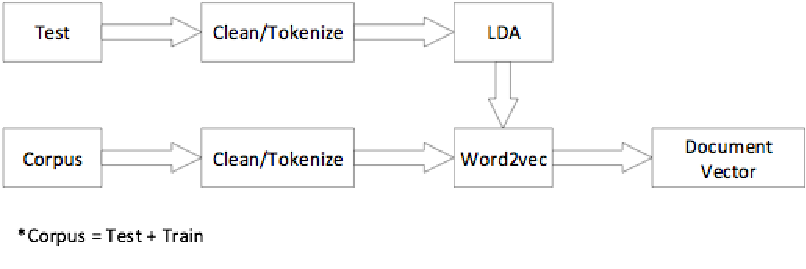
\includegraphics[scale=.58]{figs/fig7.pdf}
	\caption{Word2vec+LDA General Representation}
	\label{fig7}
\end{figure}

As indicated in Figure \ref{fig7}, the corpus and test data was used separately during training. For instance, if the test data is 1150 news dataset then the corpus data is constituted with 1150 news + 3000 tweets + 9127 tweets + Ttc 3600 + 10 million tweets datasets. The corpus data must include the test data due to capture topic words by word embedding methods.

\subsection{Parameter Selection}

The parameter selection is important for modelling an optimum hypothesis in both machine learning and deep learning. This section the optimum parameter settings are summarized for the algorithms which are used in our experiments.

Word2vec and Doc2vec models use CBOW and DM models respectively, with the parameters: vector size is 100, window length is 5, min count is 1, training epochs are 5 and negative samples are 5.

The parameters used in LDA are:  topic number is set to 10; the number of passes is set to 1000; the parameter $\alpha$ is set to 50/number of topics; the parameter $\beta$ is set to 0.01. The perplexity \citep{ref5} which measures the ability of a LDA model to generalize to unseen data is used to investigate the impact of different numbers of topics on the proposed approach. It is observed that, our method achieves the best overall performance when the topic number is 10 for both Turkish and English datasets as it is seen in Table \ref{tab3} and Table \ref{tab4} respectively.


\begin{table}[width=.9\linewidth,cols=4,pos=h]
	\caption{Perplexity of LDA with different numbers of topics for Turkish datasets}	\label{tab3}
	\begin{tabular*}{\tblwidth}{@{} LLLLL@{} }
		\toprule
		\textbf{}   & \textbf{10 Topics} & \textbf{20 Topics} & \textbf{50 Topics} & \textbf{100 Topics} \\ 
		\midrule
		1150News & -48.56             & -55.67             & -73.77             & -64.83              \\ 
		3000Tweet  & -64.62             & -70.98             & -77.56            & -80.52             \\ 
		9127Tweet   & -35.95             & -40.14             & -41.76             & -42.84              \\ 
		Ttc-3600 & -30.87             & -35.52             & -40.28             & -36.11              \\  
		\bottomrule
	\end{tabular*}
\end{table}



\begin{table}[width=.9\linewidth,cols=4,pos=h]
	\caption{Perplexity of LDA with different numbers of topics for English datasets}	\label{tab4}
	\begin{tabular*}{\tblwidth}{@{} LLLLL@{} }
		\toprule
	 	\textbf{}   & \textbf{10 Topics} & \textbf{20 Topics} & \textbf{50 Topics} & \textbf{100 Topics} \\ 
		\midrule
		Archeage & -38.42             & -46.34             & -61.64             & -73.85              \\ 
		Iphone6  & -65.46             & -73.34             & -100.65            & -101.03             \\ 
		Hobbit   & -48.49             & -58.44             & -76.16             & -85.92              \\ 
		Sts-gold & -50.51             & -61.42             & -79.10             & -90.83              \\  
		\bottomrule
	\end{tabular*}
\end{table}



\section{Experimental Results}

In our experiments, LDA is used to extract latent topics and word2vec is used to extract word vectors simultaneously. For both LDA and Word2vec we use Gensim implementations \citep{ref20}. 

The proposed method is applied to create Topic Words Vectors, which we name TopWord2vec, of the documents in the datasets. After that, the latent document representations which is learnt by TopWord2vec approach is used in classification experiments with well-known supervised learning algorithms such as Linear SVM, KNN (k=3), Random Forest, Bernoulli Bayes and Logistic Regression.

The classification results are presented using accuracy as our main evaluation metric. This is due to the fact that F-measure and accuracy values from the experiments are very close. Table \ref{tab5} shows the classification results of SVM algorithm for Turkish news and tweet datasets.
\begin{table}[width=.9\linewidth,cols=4,pos=h]
	\caption{Classification accuracies with SVM}	\label{tab5}
	\begin{tabular*}{\tblwidth}{@{} LLLL@{} }
		\toprule
		\multirow{2}{*}{\textbf{Datasets}} & \multicolumn{2}{L}{\textbf{Classification Accuracies (\%)}} \\ \cmidrule{2-3} 
		& \textbf{TopWord2vec}            & \textbf{Doc2vec}           \\ 
		\midrule
		1150News                           & 90.26                              & 88.43                         \\ 
		3000Tweet                          & 58.79                              & 47.60                         \\ 
		9127Tweet                          & 79.84                              & 74.82                         \\ 
		Ttc-3600                           & 87.39                              & 86.50                         \\ 
		\bottomrule
	\end{tabular*}
\end{table}

When Table \ref{tab5} is examined, it can be seen that the results obtained by using TopWord2vec vector in SVM is better than the results obtained by using Doc2vec in SVM for all Turkish datasets.

Table \ref{tab6} shows the results of KNN algorithm, and the results indicate that, KNN algorithm provided a minimum increase of 6\% in Turkish datasets by using proposed TopWord2vec instead of Doc2vec.
\begin{table}[width=.9\linewidth,cols=4,pos=h]
	\caption{Classification accuracies with KNN}	\label{tab6}
	\begin{tabular*}{\tblwidth}{@{} LLLL@{} }
		\toprule
		\multirow{2}{*}{\textbf{Datasets}} & \multicolumn{2}{L}{\textbf{Classification Accuracies (\%)}} \\ \cmidrule{2-3} 
		& \textbf{TopWord2vec}            & \textbf{Doc2vec}           \\ 
		\midrule
		1150News                           & 88.52                              & 82.96                         \\ 
		3000Tweet                          & 49.36                              & 33.80                         \\ 
		9127Tweet                          & 77.45                              & 64.91                         \\ 
		Ttc-3600                           & 84.56                              & 78.42                         \\ 
		\bottomrule
	\end{tabular*}
\end{table}

The classification results of Random Forrest algorithm are shown in Table \ref{tab7}. The proposed method gives better classification results than doc2vec model. The Random Forrest algorithm provided a minimum increase of 6\% by using TopWord2vec in Turkish datasets.
\begin{table}[width=.9\linewidth,cols=4,pos=h]
	\caption{Classification accuracies with Random Forest}	\label{tab7}
	\begin{tabular*}{\tblwidth}{@{} LLLL@{} }
		\toprule
		\multirow{2}{*}{\textbf{Datasets}} & \multicolumn{2}{L}{\textbf{Classification Accuracies (\%)}} \\ \cmidrule{2-3} 
		& \textbf{TopWord2vec}            & \textbf{Doc2vec}           \\ 
		\midrule
		1150News                           & 85.04                              & 77.22                         \\ 
		3000Tweet                          & 49.23                              & 41.29                         \\ 
		9127Tweet                          & 76.21                              & 70.06                         \\ 
		Ttc-3600                           & 82.61                              & 74.19                         \\ 
		\bottomrule
	\end{tabular*}
\end{table}

Table \ref{tab8} shows linear Bernoulli Bayes algorithm classification results by using Turkish news and tweet data. As in other classification algorithms, TopWord2vec gives better results than Doc2vec. There is no increase in the datasets of 1150News and Ttc-3600 on the Bernoulli Bayes algorithm, but an increase of 3000Tweet and 9127Tweet data has been observed.

\begin{table}[width=.9\linewidth,cols=4,pos=h]
	\caption{Classification accuracies with Bernoulli Naive Bayes}	\label{tab8}
	\begin{tabular*}{\tblwidth}{@{} LLLL@{} }
		\toprule
		\multirow{2}{*}{\textbf{Datasets}} & \multicolumn{2}{L}{\textbf{Classification Accuracies (\%)}} \\ \cmidrule{2-3} 
		& \textbf{TopWord2vec}            & \textbf{Doc2vec}           \\ 
		\midrule
		1150News                           & 87.48                              & 87.13                         \\ 
		3000Tweet                          & 53.91                              & 40.43                         \\ 
		9127Tweet                          & 76.33                              & 64.48                         \\ 
		Ttc-3600                           & 81.31                              & 80.89                         \\ 
		\bottomrule
	\end{tabular*}
\end{table}

Table \ref{tab9} shows the classification results of linear Logistic Regression algorithm by using Turkish news and tweet data. There is no increase in the Ttc-3600 dataset on the Logistic Regression algorithm, but an increase in other datasets has been observed.


\begin{table}[width=.9\linewidth,cols=4,pos=h]
	\caption{Classification accuracies with Logistic Regression}	\label{tab9}
	\begin{tabular*}{\tblwidth}{@{} LLLL@{} }
		\toprule
		\multirow{2}{*}{\textbf{Datasets}} & \multicolumn{2}{L}{\textbf{Classification Accuracies (\%)}} \\ \cmidrule{2-3} 
		& \textbf{TopWord2vec}            & \textbf{Doc2vec}           \\ 
		\midrule
		1150News                           & 89.13                              & 84.09                         \\ 
		3000Tweet                            & 58.99                              & 47.26                         \\ 
		9127Tweet                             & 79.33                              & 75.41                         \\ 
		Ttc-3600                           & 86.50                              & 86.28                         \\ 
		\bottomrule
	\end{tabular*}
\end{table}

In general, when the classification results for Turkish datasets are examined, it is seen that, the SVM algorithm produces the superior results when it is used with TopWord2vec instead of Doc2vec

Table \ref{tab10} shows the linear SVM algorithm classification results by using English tweet data. While there is no increase in Archeage and Sts-gold data, there is a decrease in Iphone6 and Hobbit datasets.

\begin{table}[width=.9\linewidth,cols=4,pos=h]
	\caption{Classification accuracies with SVM}	\label{tab10}
	\begin{tabular*}{\tblwidth}{@{} LLLL@{} }
		\toprule
		\multirow{2}{*}{\textbf{Datasets}} & \multicolumn{2}{L}{\textbf{Classification Accuracies (\%)}} \\ \cmidrule{2-3} 
		& \textbf{TopWord2vec}            & \textbf{Doc2vec}           \\ 
		\midrule
		Archeage                           & 77.34                              & 75.15                         \\ 
		Iphone6                            & 71.75                              & 73.11                         \\ 
		Hobbit                             & 77.12                              & 73.73                         \\ 
		Sts-gold                           & 79.12                              & 78.17                         \\ 
		\bottomrule
	\end{tabular*}
\end{table}

Table \ref{tab11} shows the linear KNN algorithm classification results by using English tweet data. TopWord2vec gives better results than Doc2vec. In particular, there was an 9\% increase in Archeage dataset.

\begin{table}[width=.9\linewidth,cols=4,pos=h]
	\caption{Classification accuracies with KNN}	\label{tab11}
	\begin{tabular*}{\tblwidth}{@{} LLLL@{} }
		\toprule
		\multirow{2}{*}{\textbf{Datasets}} & \multicolumn{2}{L}{\textbf{Classification Accuracies (\%)}} \\ \cmidrule{2-3} 
		& \textbf{TopWord2vec}            & \textbf{Doc2vec}           \\ 
		\midrule
		Archeage                           & 74.80                              & 66.06                         \\ 
		Iphone6                            & 73.08                              & 71.82                         \\ 
		Hobbit                             & 75.05                              & 70.08                         \\ 
		Sts-gold                           & 73.76                              & 69.32                         \\ 
		\bottomrule
	\end{tabular*}
\end{table}

Table \ref{tab12} shows the linear Random Forest algorithm classification results by using English tweet data. TopWord2vec gives better results than Doc2vec. In particular, there was an 11\% increase in Hobbit dataset.

\begin{table}[width=.9\linewidth,cols=4,pos=h]
	\caption{Classification accuracies with Random Forest}	\label{tab12}
	\begin{tabular*}{\tblwidth}{@{} LLLL@{} }
		\toprule
		\multirow{2}{*}{\textbf{Datasets}} & \multicolumn{2}{L}{\textbf{Classification Accuracies (\%)}} \\ \cmidrule{2-3} 
		& \textbf{TopWord2vec}            & \textbf{Doc2vec}           \\ 
		\midrule
		Archeage                           & 72.42                              & 68.05                         \\ 
		Iphone6                            & 70.43                              & 66.16                         \\ 
		Hobbit                             & 76.22                              & 65.13                         \\ 
		Sts-gold                           & 73.11                              & 69.47                         \\ 
		\bottomrule
	\end{tabular*}
\end{table}

Table \ref{tab13} shows the linear Bernoulli Bayes algorithm classification results by using English tweet data. TopWord2vec gives better results than Doc2vec. In particular, there was a 12\% increase in Iphone6 dataset.


\begin{table}[width=.9\linewidth,cols=4,pos=h]
	\caption{Classification accuracies with Bernoulli Naive Bayes}	\label{tab13}
	\begin{tabular*}{\tblwidth}{@{} LLLL@{} }
		\toprule
		\multirow{2}{*}{\textbf{Datasets}} & \multicolumn{2}{L}{\textbf{Classification Accuracies (\%)}} \\ \cmidrule{2-3} 
		& \textbf{TopWord2vec}            & \textbf{Doc2vec}           \\ 
		\midrule
		Archeage                           & 71.00                              & 63.88                         \\ 
		Iphone6                            & 70.64                              & 61.28                         \\ 
		Hobbit                             & 72.04                              & 62.04                         \\ 
		Sts-gold                           & 73.41                              & 69.47                         \\ 
		\bottomrule
	\end{tabular*}
\end{table}

Table \ref{tab14} shows the linear Logistic Regression algorithm classification results by using English tweet data. TopWord2vec gives better results than Doc2vec. There was no increase in the Iphone6 dataset, but an increase in other datasets was observed.

\begin{table}[width=.9\linewidth,cols=4,pos=h]
	\caption{Classification accuracies with Logistic Regression}	\label{tab14}
	\begin{tabular*}{\tblwidth}{@{} LLLL@{} }
		\toprule
		\multirow{2}{*}{\textbf{Datasets}} & \multicolumn{2}{L}{\textbf{Classification Accuracies (\%)}} \\ \cmidrule{2-3} 
		& \textbf{TopWord2vec}            & \textbf{Doc2vec}           \\ 
		\midrule
			Archeage                           & 77.90                              & 75.44                         \\ 
			Iphone6                            & 71.18                              & 70.66                         \\ 
			Hobbit                             & 78.50                              & 71.24                         \\ 
			Sts-gold                           & 79.40                              & 77.29                         \\ 
		\bottomrule
	\end{tabular*}
\end{table}


In general, document representations, e.g. document vectors obtained by our proposed approach TopWord2vec yields better classification results by a wide range of classification algorithms compare to the doc2vec representations on a large number and variety of text classification datasets in two different languages; English and Turkish.

Yet another benefit of our proposed approach is better computational time complexity. When we measure the training times (Table \ref{tab15}) we see that it is faster to train TopWord2vec model.


\begin{table}[width=.9\linewidth,cols=4,pos=h]
	\caption{Training time in minutes}	\label{tab15}
	\begin{tabular*}{\tblwidth}{@{} LLLL@{} }
		\toprule
			\textbf{}       & \textbf{TopWord2vec} & \textbf{Doc2vec} \\ 
		\midrule
			Turkish Dataset & 25 m.                & 367 m.           \\ 
			English Dataset & 3 m.                 & 14 m.            \\ 
		\bottomrule
	\end{tabular*}
\end{table}

\section{Conclusion}

In this paper, we propose a new document vector representation based on topic and word distributions of a given document combined with word embedding vectors of the words of this document. LDA and Word2Vec methods are integrated for the proposed document vector which is called as TopWord2vec. The proposed algorithm to create document vectors not only make use of  co-occurrence relations between words, but also considers the theme of the document and words which are good representatives of these themes. The experimental results show that document representations, e.g. document vectors obtained by our proposed approach TopWord2vec yields better classification results by a wide range of classification algorithms on a large number and variety of text classification datasets in two different languages; English and Turkish, compare to the doc2vec representations.

As a future plan, we aim to analyze whether the TopWord2vec representation improves the performance of information retrieval from the documents. Additionally, we also aim to implement TopWord2vec document vectors in unsupervised machine learning models. 

\section{ Acknowledgement}

This work is supported in part by The Scientific and Technological Research Council of Turkey (TÜBİTAK) grant number 116E047. Points of view in this document are those of the authors and do not necessarily represent the official position or policies of the TÜBİTAK.

\bibliographystyle{cas-model2-names}

% Loading bibliography database
\bibliography{cas-refs}



\end{document}



